% Le but de ce travail de bachelor consiste, premièrement, de construire un système sécurité au système de pinces optiques par laser afin de faciliter son utilisation au quotidien. Le système est équipé d'un laser de classe 3B (puissance 40mW) continu et peut donc engendrer de graves problèmes oculaires. L'objectif est de concevoir une protection correspondant à un système de classe , adapté à une utilisation sans lunettes de protection laser.

% Deuxièmement, une proposition d'expérience avec un mode d'emploi compact est proposé pour le cours de NANO (Nanotechnologies et Applications Industrielles), un cours à choix de 3\ieme{} année. La documentation actuelle fournie par le fabricant est volumineuse et peu adaptée pour une utilisation en laboratoire pour des étudiants.

% Le troisième objectif est de développer une application graphique intégrant des fonctionnalités de traitement d'image pour automatiser l'utilisation de la pince optique, par exemple, pour trier des particules de manière automatisée ou de réaliser des assemblages en milieu liquide. Cette démarche de codage permet de mettre en pratique les outils acquis tout au long du cursus de bachelor.

% Ce projet vise donc à rendre l'expérience plus sûre, plus accessible pour tout utilisateur et permet une automatisation partielle du processus de manipulation optique des particules.
\section{Système de la pince optique}

Le système de pinces optiques portables, Portable Optical Tweezers, est un dispositif qui permet de déplacer des microobjets grâce à un faisceau laser focalisé. L'entreprise américaine qui vends ce système est Thorlabs. La citation suivante est traduite de l'anglais: \guillemotleft{}~Thorlabs conçoit et fabrique des produits dans les domaines de la fibre optique, des lasers, de l'instrumentation optique, de l'optomécanique, de la photonique et de l'isolation contre les vibrations~\guillemotright{}\cite{thorlabsWikipedia}.

\subsection{Principe de fonctionnement d'une pince optique}

La théorie décrite ci-dessous s'appuie sur le chapitre 3 du manuel du système \cite{manualPortableOpticalTweezers}.

Le principe des pinces optiques repose sur l'interaction entre un faisceau laser focalisé (profil gaussien, mode \gls{tem00}) et une petite particule diélectrique, typiquement une bille en polystyrène d'environ 1~\textmu m de diamètre. Cela génère deux forces :
\begin{itemize}[label=\textbullet]
    \item La force de gradient (\textit{gradient force}), qui agit vers les zones de plus forte intensité lumineuse, c'est-à-dire vers le foyer du faisceau.
    \item La force de diffusion (\textit{scattering force}), qui pousse la particule dans la direction de la propagation du faisceau.
\end{itemize}
Pour qu'une particule soit piégée de manière stable, il faut que la force du gradient soit plus grande que la force de diffusion.

Des modèles simples permettent d'expliquer le fonctionnement des pinces optiques en considérant deux cas limites : le régime de Rayleigh ($R \ll \lambda$) et le régime de Mie ($R \gg \lambda$), selon la taille relative de la particule par rapport à la longueur d'onde du laser.
Cependant, dans la plupart des systèmes réels, on opère dans un régime intermédiaire ($R \approx \lambda$), qui nécessite des approches théoriques plus complexes (comme la diffusion de Lorentz-Mie généralisée ou la théorie de la matrice T)~\cite{epflExplanationOpticalTweezers}.
L'étude des régimes extrêmes reste toutefois utile pour mieux comprendre les principes du piégeage optique.

Le régime de Rayleigh permet de comprendre ce principe physique.

Dans ce régime, on peut considérer la bille comme un ensemble de petits dipôles polarisables. Le champ électrique du laser induit un moment dipolaire dans chacun d'eux. Comme le champ est pratiquement uniforme sur la bille (car elle est très petite), tous les dipôles sont polarisés de la même manière. Ceci permet de représenter la bille comme un seul dipôle global, dont la polarisation dépend directement du champ électrique local.

\begin{minipage}[c]{0.55\textwidth}
    L'énergie potentielle de ce dipôle dans le champ électrique est proportionnelle à l'intensité lumineuse. De ce fait, une force apparaît, dirigée vers les zones de plus forte intensité : c'est la force de gradient, qui permet de ramener la particule vers le centre du faisceau.

    En parallèle, la force de diffusion provient de la diffusion de la lumière : le faisceau est en partie absorbé et réémis par la particule, ce qui la pousse dans le sens de propagation du faisceau. Cette force est également proportionnelle à l'intensité lumineuse, mais elle agit dans le sens opposé à celui du piégeage.
\end{minipage}\hfill
\begin{minipage}[c]{0.4\textwidth}
    \begin{figure}[H]
        \begin{center}
            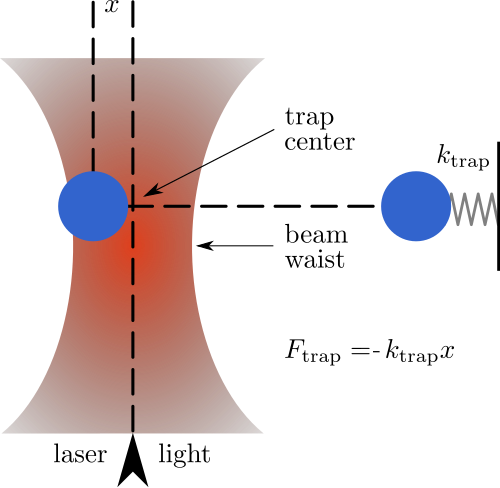
\includegraphics[width=0.9\textwidth]{assets/figures/Introduction/optical_tweezer_theorie.png}
        \end{center}
        \captionof{figure}{Principe de piégeage d'une particule dans un faisceau laser~\cite{wikipedia_opticalTweezer}}
        \label{optical_tweezer_theorie}
    \end{figure}
\end{minipage}

Enfin, les formules des deux forces montrent qu'elles dépendent toutes deux des caractéristiques du faisceau laser, du milieu et de l'indice de réfraction de la particule.

Les formules de ces forces dans le régime de Rayleigh (\( R \ll \lambda \)) sont les suivantes :


\begin{equation}
    \vec{F}_{\text{grad}} = \frac{2\pi \alpha}{c n_m^2} \nabla I
\end{equation}
\myequations{Force de gradient exercée sur une particule polarisable dans un champ électrique non uniforme.}

\textbf{Légende :}
\begin{itemize}[label=\textbullet]
    \item \( \vec{F}_{\text{grad}} \) : force de gradient
    \item \( \alpha \) : polarisabilité de la particule, donnée par \( \alpha = n_m^2 R^3 \left(\frac{m^2 - 1}{m^2 + 2}\right) \)
    \item \( c \) : vitesse de la lumière dans le vide
    \item \( n_m \) : indice de réfraction du milieu
    \item \( \nabla I \) : gradient de l'intensité lumineuse
    \item \( R \) : rayon de la particule
    \item \( m = \frac{n_p}{n_m} \) : rapport des indices de réfraction de la particule (\( n_p \)) et du milieu (\( n_m \))
\end{itemize}

\begin{equation}
    \vec{F}_{\text{scatt}} = \frac{\sigma n_m}{c} I
\end{equation}
\myequations{Force de diffusion due à l'impulsion du faisceau lumineux.}

\textbf{Légende :}
\begin{itemize}[label=\textbullet]
    \item \( \vec{F}_{\text{scatt}} \) : force de diffusion
    \item \( \sigma \) : section efficace de diffusion, donnée par \( \sigma = \frac{128\pi^5 R^6}{3 \lambda^4} \left( \frac{m^2 - 1}{m^2 + 2} \right)^2 \)
    \item \( I \) : intensité lumineuse incidente
    \item \( \lambda \) : longueur d'onde du laser
\end{itemize}

\newpage
\subsection{Description du système}
La Figure~\ref{chemin_laser_caméra} montre le trajet parcouru par le laser (\textcolor{red}{en rouge}), ainsi que du microscope vers la caméra (\textcolor[RGB]{0, 120, 0}{en vert}).
\begin{figure}[H]
    \begin{center}
        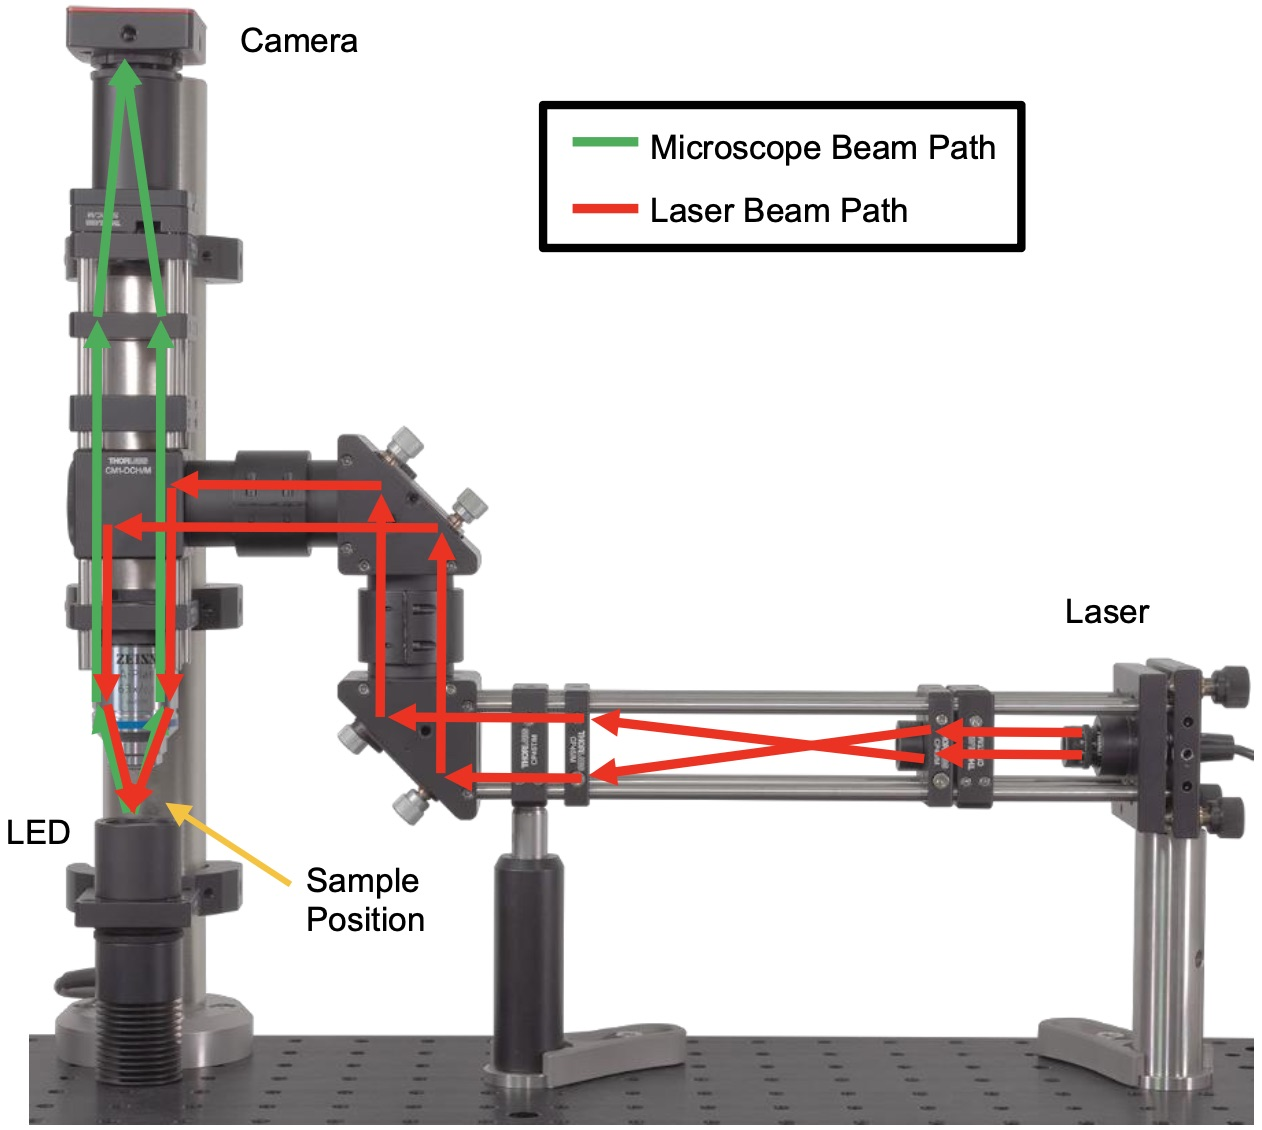
\includegraphics[width=0.7\textwidth]{assets/figures/Introduction/chemin_laser_camera.jpeg}
    \end{center}
    \caption{Trajet du laser et du microscope (image issue de la page 3 du manuel du système \cite{manualPortableOpticalTweezers})}
    \label{chemin_laser_caméra}
\end{figure}

La Figure~\ref{kit_vierge} correspond à l'état du système reçu lors du premier jour de TB. Le système a été monté par un assistant du laboratoire COMATEC-LANS.

\begin{figure}[H]
    \begin{center}
        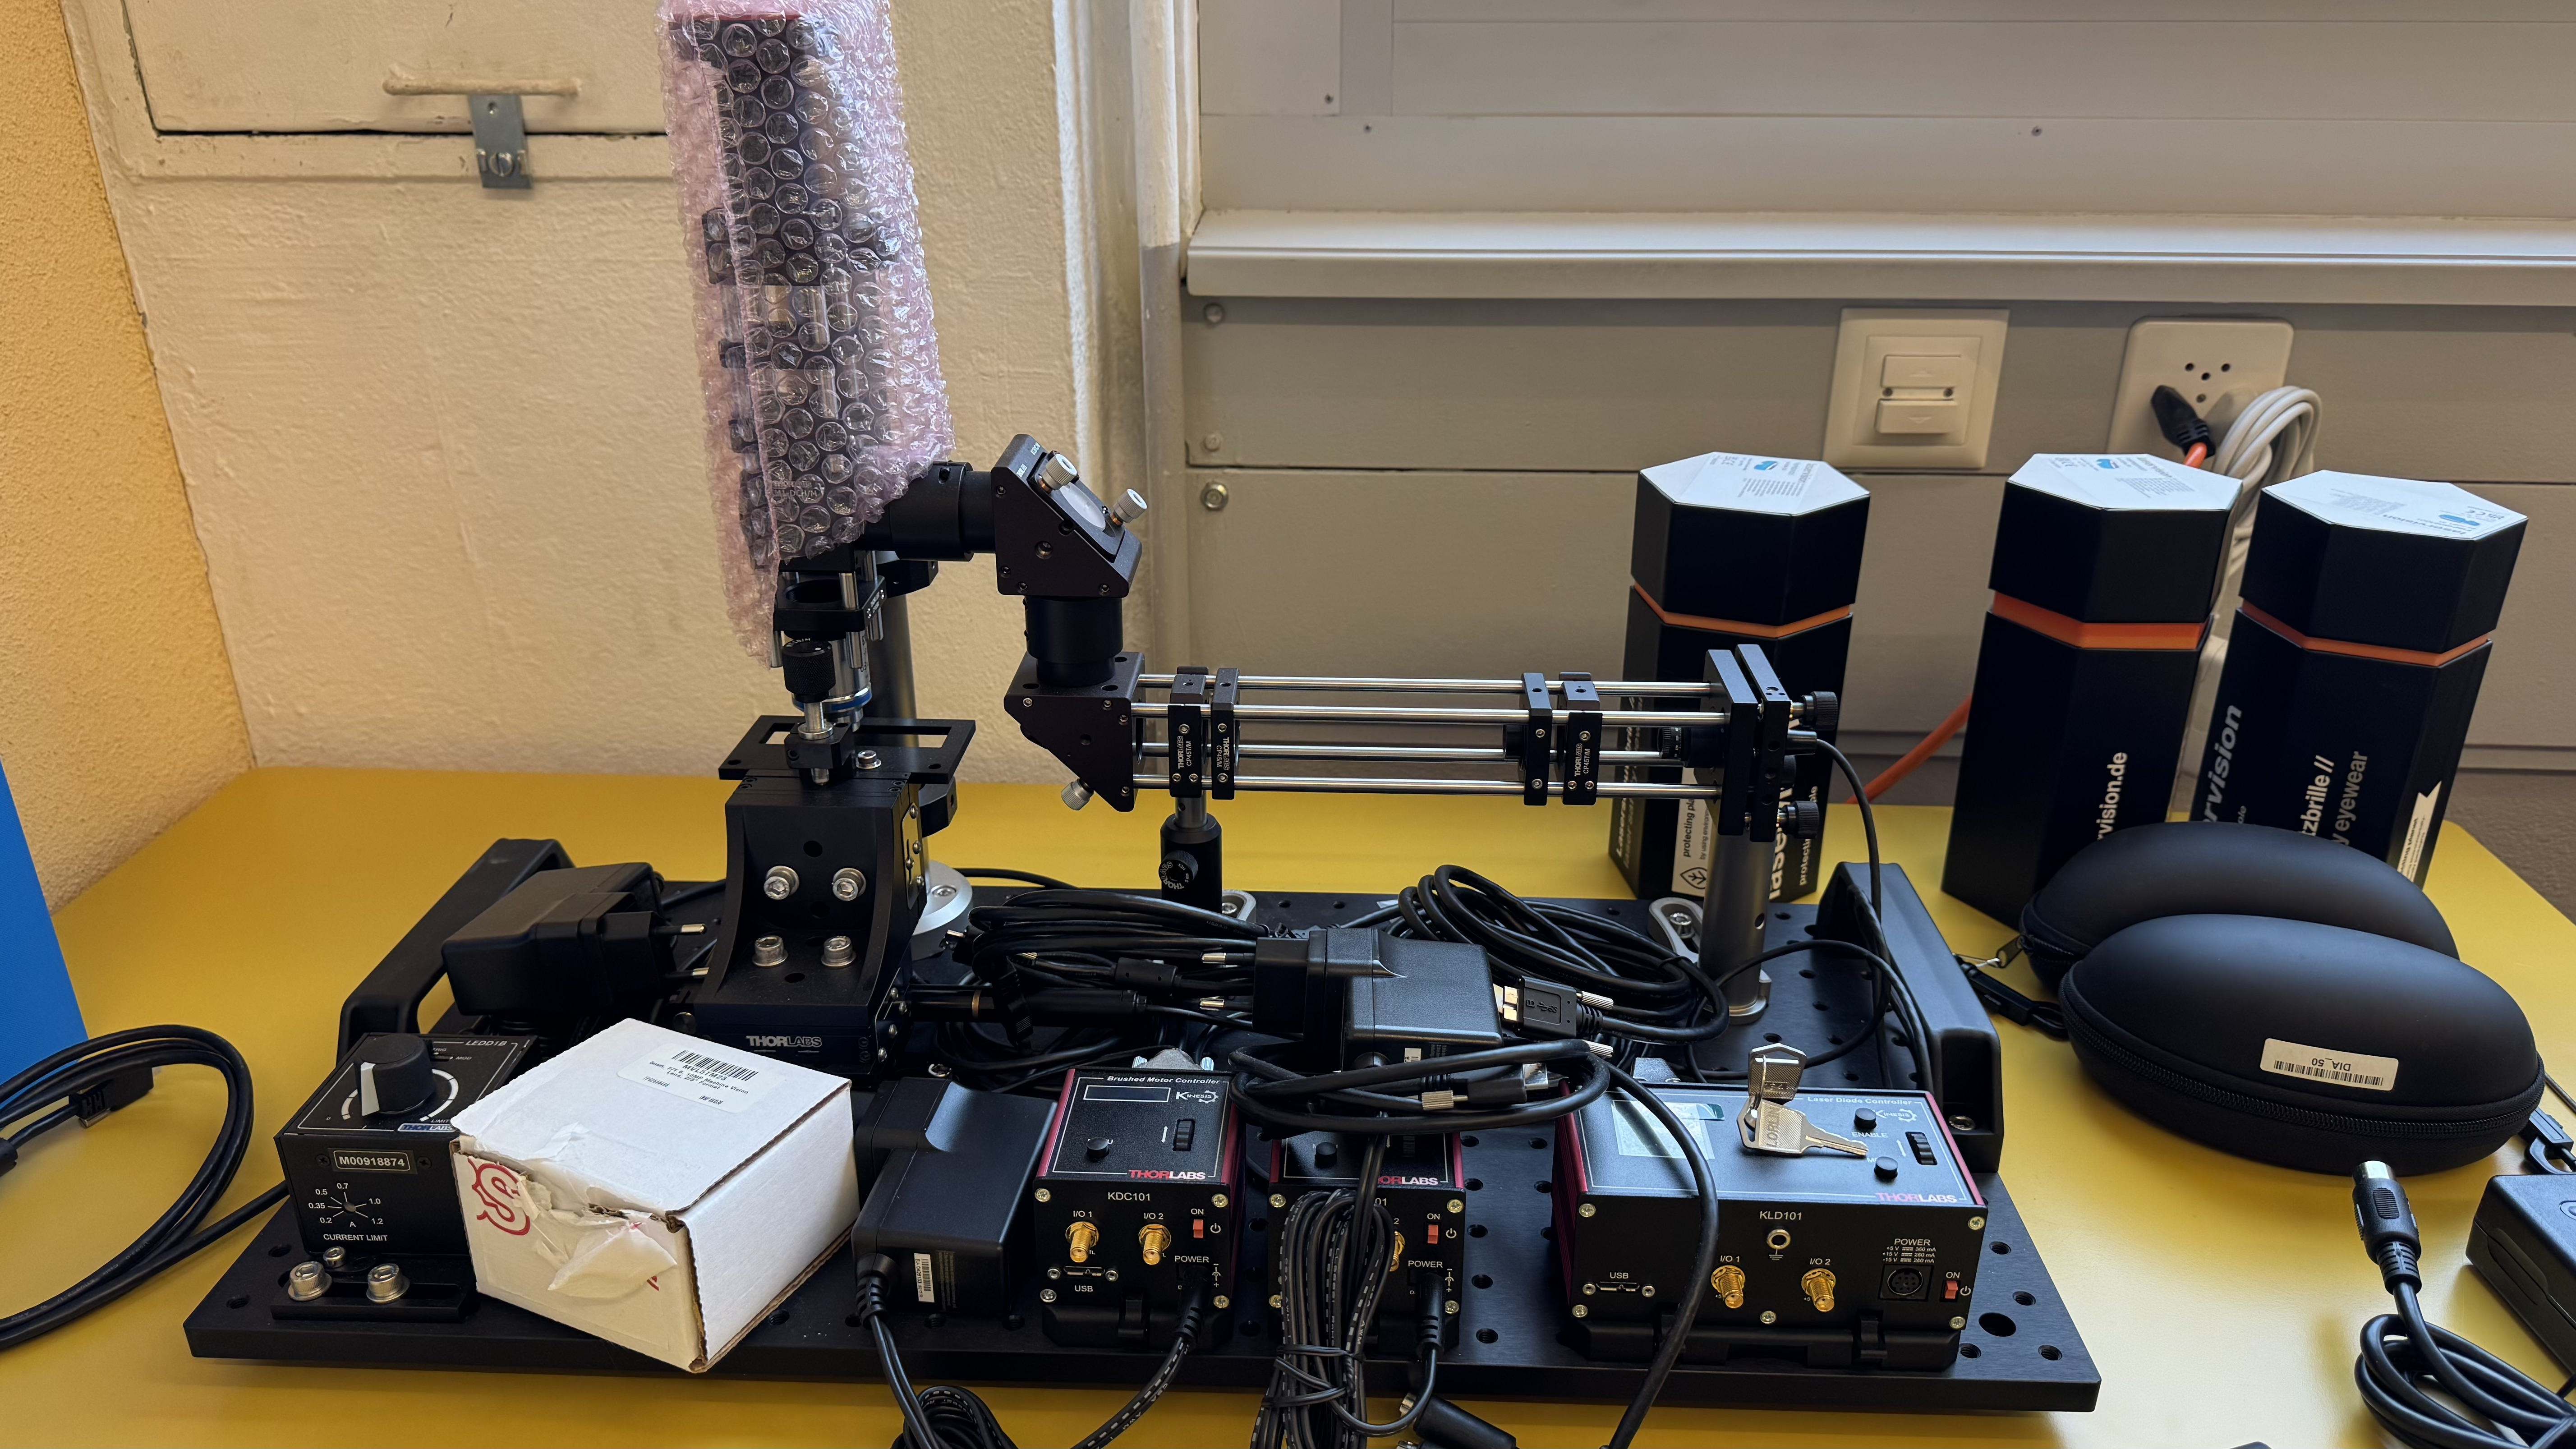
\includegraphics[width=0.7\textwidth]{assets/figures/Introduction/kit_vierge.jpeg}
    \end{center}
    \caption{Système Portable Optical Tweezers de Thorlabs}
    \label{kit_vierge}
\end{figure}

\newpage
Une représentation 3D du système, accompagnée de légendes pour chaque composant, a été réalisé par mes soins.\label{modelisation_3D} Ce modèle CAO permet une clareté et une compréhension plus rapide des différents éléments. Les différentes modélisations 3D des composants ont directement été pris du site Thorlabs \cite{portableOpticalTweezers}, dans l'onglet \guillemotleft Component List\guillemetright. Je me suis chargé de les intégrer dans un seul fichier CAO et d'en effectuer l'assemblage. Voir la Figure~\ref{kit_CAO_vierge_annote}.

\begin{figure}[H]
    \begin{center}
        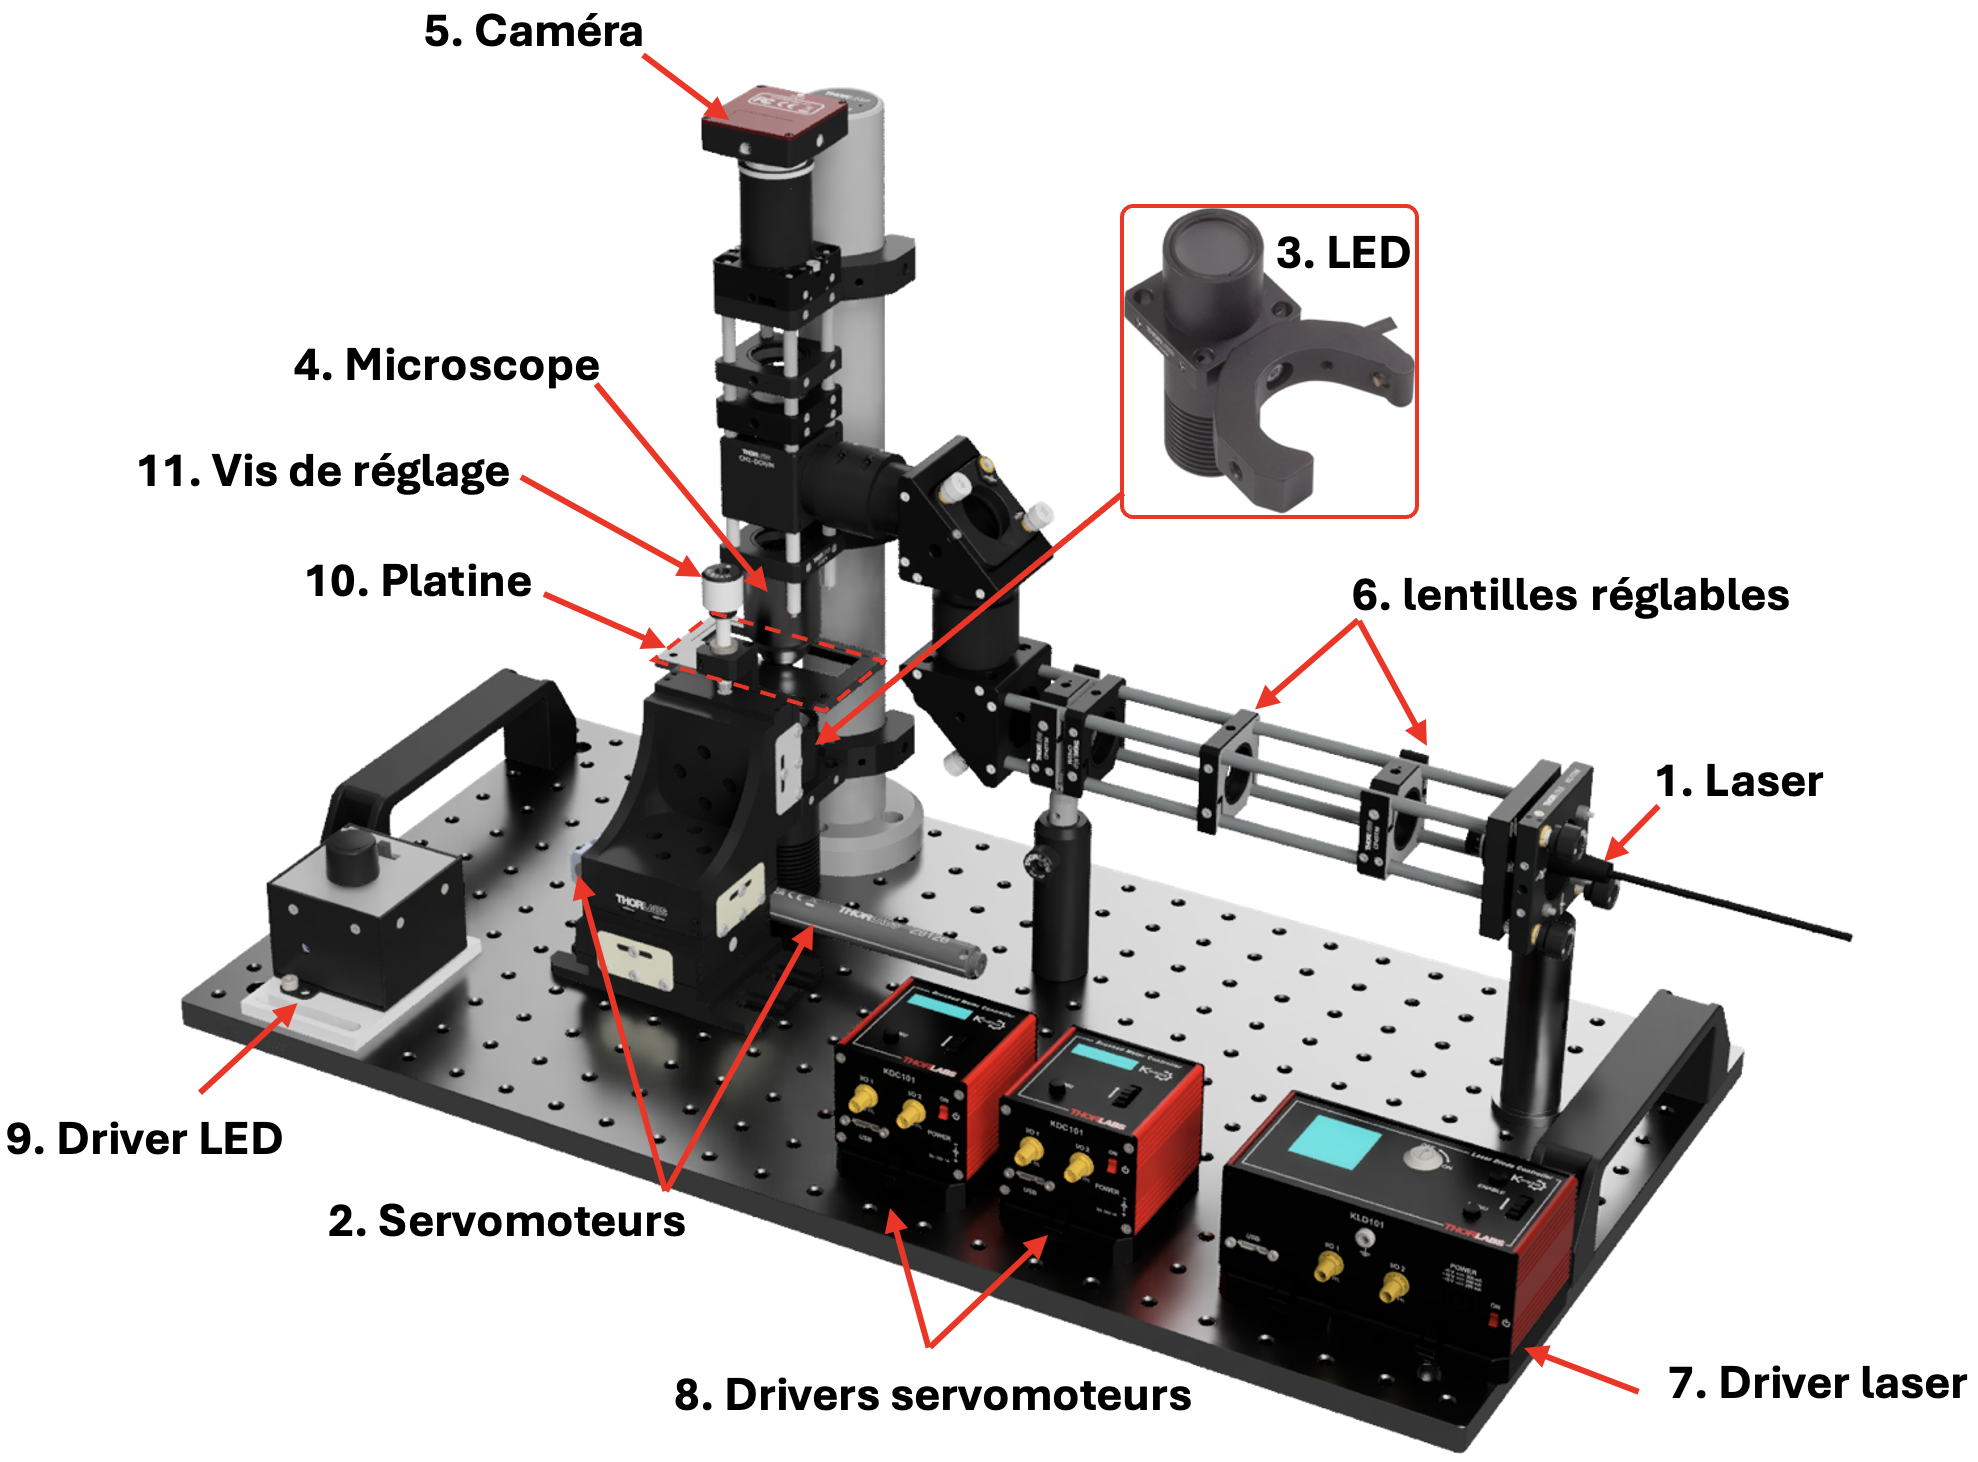
\includegraphics[width=\textwidth]{assets/figures/Introduction/Kit_CAO_vierge_annote.png}
    \end{center}
    \caption{CAO du système avec annotations des principaux composants}
    \label{kit_CAO_vierge_annote}
\end{figure}

\begin{enumerate}
    \item Laser de classe 3B, d'une longueur d'onde 658 nm (couleur rouge visible) avec une puissance maximale de 40 mW.
    \item Les servomoteurs permettent de déplacer la platine en X Y.
    \item La LED permet un réglage manuel de l'éclairage.
    \item Microscope équipé d'un objectif avec un grossissement de $63\times$ et une ouverture numérique de 0,8.
    \item Caméra couleur de 1,6 mégapixel.
    \item Lentilles réglables afin de modifier la hauteur de la mise au point du laser.
    \item Ce driver permet de piloter le laser, soit directement avec les boutons intégrés, soit via l'application Kinesis \cite{kinesisSoftware} pour une meilleure ergonomie.
    \item Ces drivers permettent le pilotage des servomoteurs, soit directement avec les boutons intégrés, soit via l'application Kinesis pour une meilleure ergonomie.
    \item Ce driver permet de faire varier l'intensité lumineuse de la LED.
    \item La platine permet d'accueillir l'échantillon que l'on veut analyser.
    \item La vis de réglage, de pas très fin, permet d'ajuster précisement la hauteur souhaitée de la platine.
\end{enumerate}

\section{Objectifs}

Les différents objectifs de ce travail de bachelor sont listés ci-dessous :
\begin{enumerate}
    \item Mettre en service le système : câblage, calibration du laser
    \item Conception de protection contre le laser afin d'apporter plus de sécurité lors de l'utilisation du système
    \item Élaboration d'une notice de laboratoire compacte pour utiliser simplement le système
    \item Réalisation d'une application avec interface graphique visant à pouvoir combiner les 2 applications proposées par Thorlabs, détecter automatiquement des particules, ainsi que les déplacer de façon autonome.
          % \item Effectuer des tests de déplacements de microbilles dans différents milieux, de différentes viscosités, dans différents types de réservoirs ainsi que de multiples canaux.
          % \item Analyses expérimentales des forces de déplacement en fonction de la viscosité des fluides
\end{enumerate}

\subsection{Mise en service du système}

La première partie consiste à mettre en service le système. Il faut alimenter les différents drivers qui contrôlent les moteurs, la LED ainsi que le driver lié au laser. Viens ensuite la procédure de calibration du laser, ainsi que l'installation des logiciels permettant de contrôler; d'une part les drivers des moteurs, et d'autre part le driver du laser.

\subsection{Protections contre le laser}
L'utilisation de lasers puissants dans un système expérimental doit être une des premières préoccupations de la personne responsable.

Dans le cadre de ce TB, deux niveaux de protection ont été élaborés afin de garantir au mieux la sécurité du laser :

\begin{enumerate}
    \item Le premier niveau est électrique et repose sur deux dispositifs :
          \begin{itemize}[label=\textbullet]
              \item Le système intégré interlock du driver du laser va être modifié pour fonctionner avec les protections mécaniques.
              \item Un boîtier contenant un bouton d'arrêt d'urgence ainsi qu'une clé de maintenance vont être apportés en plus dans le système interlock.
          \end{itemize}
    \item Le second niveau est mécanique et comprend deux mécanismes :
          \begin{itemize}[label=\textbullet]
              \item Le premier est située à l'entrée du faisceau laser.
              \item Le second est située vers le microscope, en fin de trajet du laser.
          \end{itemize}
\end{enumerate}
\begin{minipage}{\textwidth}
    La première protection à réaliser est située au début du laser et va devoir entourer toute la cage où le faisceau du laser passe. L'encadré en \textcolor{red}{rouge} représente l'endroit où la protection va devoir être imaginée. Voir la Figure~\ref{protection_laser_début}.

    \begin{figure}[H]
        \begin{center}
            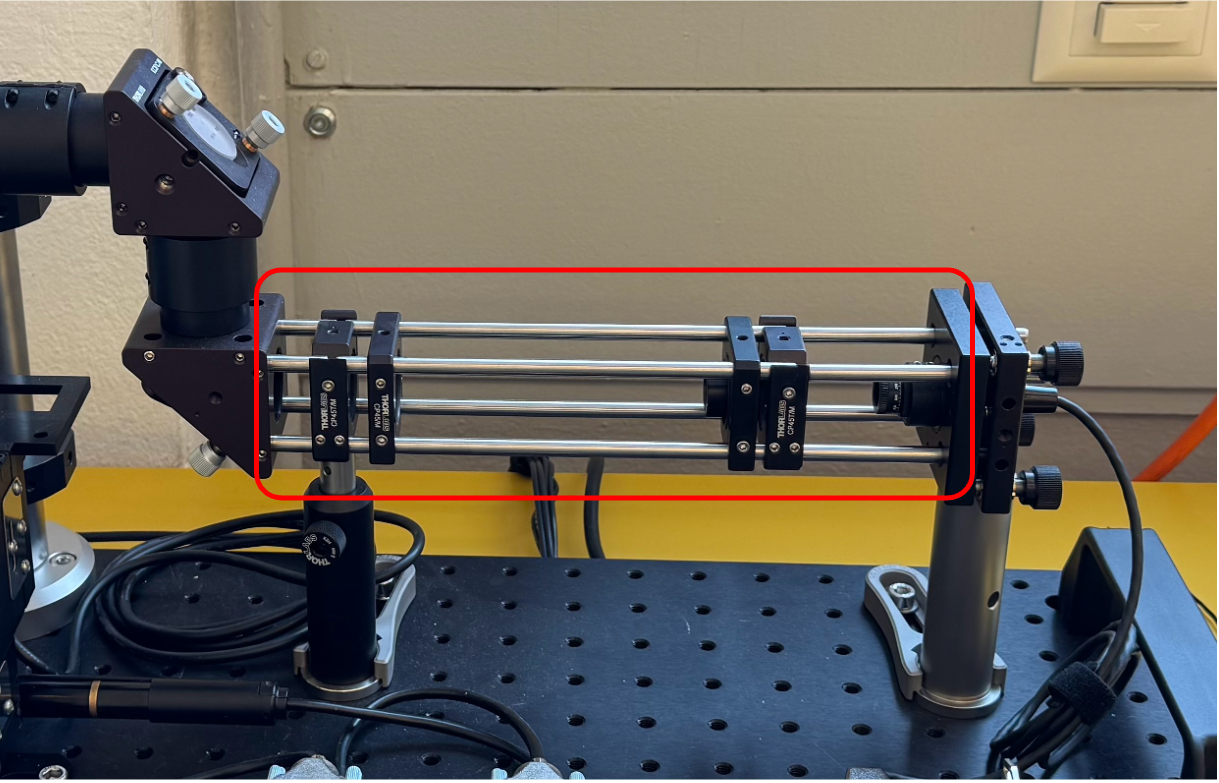
\includegraphics[width=0.5\textwidth]{assets/figures/Introduction/protection_debut_laser.png}
        \end{center}
        \captionof{figure}{Première protection située vers le laser}
        \label{protection_laser_début}
    \end{figure}
\end{minipage}

\begin{minipage}{\textwidth}
    Une deuxième protection va être faite vers le microscope, car également à cet endroit, le laser devient visible à l'oeil nu et il y'a un grand risque de se blesser. L'encadré en \textcolor{blue}{bleu} représente l'endroit où la protection va devoir être imaginée. Voir la Figure~\ref{protection_laser_fin}.
    \vspace{1em}
    \begin{figure}[H]
        \begin{center}
            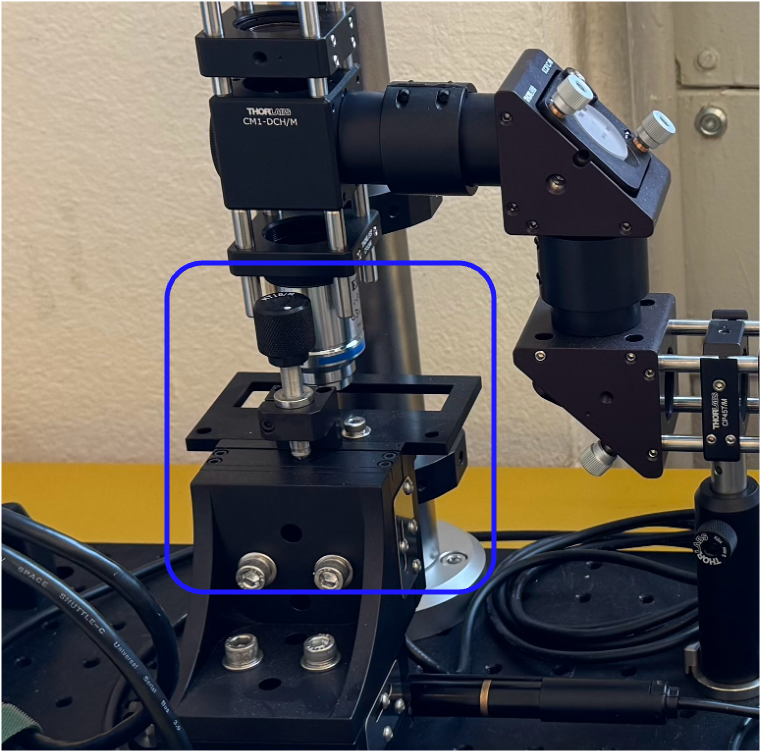
\includegraphics[width=0.5\textwidth]{assets/figures/Introduction/protection_fin_laser.png}
        \end{center}
        \captionof{figure}{Deuxième protection contre le laser située vers le microscope}
        \label{protection_laser_fin}
    \end{figure}
\end{minipage}

\vspace{1em}
Le chapitre \ref{chapter:securite_electrique} explique la partie électrique, tandis que le chapitre \ref{chapter:securite_mecanique} détaille la partie mécanique.

\subsection{Expérience et notice de laboratoire}

Un des objectifs de ce TB, consite également à créer une notice de laboratoire pour un cours à choix de 3\ieme{} année, intitulé NANO. Cette notice devra être simple à comprendre, compacte et comprendra des manipulations avec différents liquides, ainsi que des mesures pratiques. Des notices du fabricant sont accompagnées avec le système, mais sont très volumineuses, car elles doivent expliquer tout le système en détail. Ici, le but est de faire une expérience centrée uniquement sur les éléments nécessaires à la manipulation.

\subsection{Application avec interface graphique}

Cette application permettrait d'intéragir avec les deux logiciels ThorCam~\cite{thorcamSoftware} et Kinesis~\cite{kinesisSoftware}. ThorCam sert à afficher l'image en direct de la caméra, et Kinesis permet de contrôler les moteurs de translation ainsi que le laser. Le but est de rassembler ces deux outils dans un seul programme, et d'y ajouter du traitement d'image. Par exemple, on pourrait détecter automatiquement des particules dans l'image, puis les attraper et les déplacer avec le faisceau laser en contrôlant les moteurs via Kinesis.

%%if
% \section{Citations et bibliographie}
% Citer vos sources est essentiel. Avec \texttt{biblatex} vous pouvez facilement citer des articles, des livres ou des sites internet. Toutes les citations dans le texte seront automatiquement regroupées en fin de document dans la section \guillemotleft Bibliographie\guillemotright. Par exemple, citons un article d'Einstein \cite{einstein} ou le livre de Dirac \cite{dirac}.

% Parfois il peut être utile d'utiliser un gestionnaire de bibliographie. La communauté académique recommande l'outil \href{https://www.zotero.org/}{Zotero} qui permet de gérer une bibliothèque numérique d'ouvrages et de références numériques. Il permet également de générer une bibliographie compatible avec \LaTeX.

% Notez qu'il est très facile d'obtenir l'extrait \texttt{bibtex} depuis des journaux. Sélectionnez \emph{export/citation}. Si vous le pouvez choisissez \texttt{bibtex}. Dans le cas d'un format \texttt{.ris}, utilisez un convertisseur en ligne comme \href{http://www.bruot.org/ris2bib/}{ris2bib}.

% \section{Adapter votre modèle}
% Ce document n'est qu'un modèle ayant pour but de revoir les quelques avantages de \LaTeX~ et les fonctionnalités qui pourraient vous être utiles pour rédiger un rapport académique. N'hésitez pas à supprimer les parties inutiles et à adapter ce modèle à vos besoins.
%%fi